\chapter{Which are the other components of the Infrastructure that will be connected to your Analytics}

\section{Arduino Portenta H7}

Due to the presence of dual-core processors, the Arduino Portenta H7 is capable of doing high-level code execution in addition to real-time tasks simultaneously. For instance, you could simultaneously run code written in MicroPython and Arduino, and both cores could communicate to each other \cite{ArduinoH72022}. 

\bigskip

There are two primary modes of operation for the Arduino Portenta H7: standalone and host. The Portenta H7 supports both of these modes of operation. It also offers several other features and capabilities that make it useful in various applications, including machine learning support, real-time processing, and low-power mode.

\begin{figure}[h]
     \centering
     \begin{subfigure}[b]{0.49\textwidth}
         \centering
         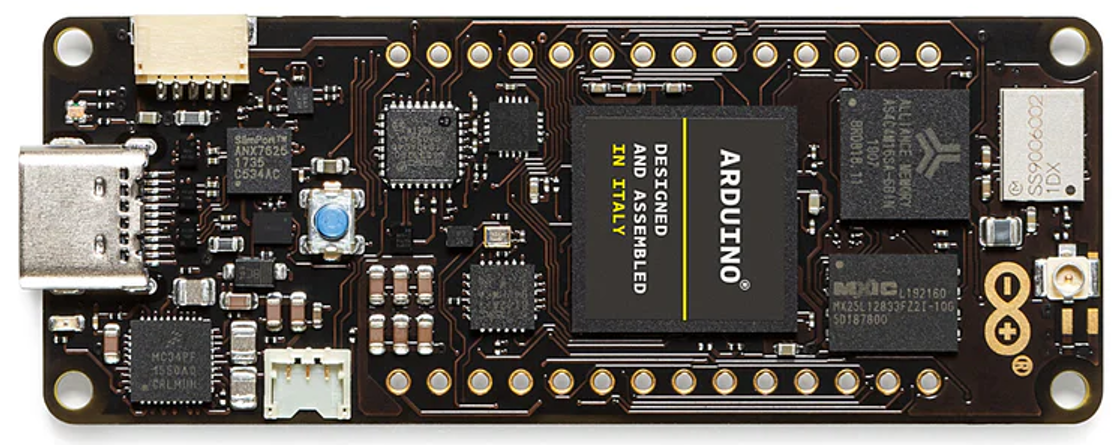
\includegraphics[scale=0.2]{Images/Arduino Portenta H7.png}
         \captionsetup{justification=centering}
         \caption{Arduino Portenta H7 \\ source: \cite{ArduinoH72022}}
         \label{fig:Arduino Portenta H7}
     \end{subfigure}
     \hfill
     \begin{subfigure}[b]{0.49\textwidth}
         \centering
         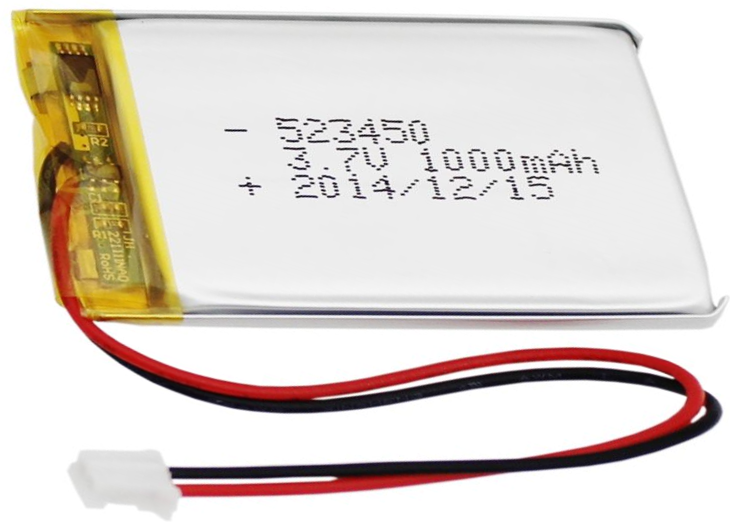
\includegraphics[scale=0.2]{Images/Li-Po Battery.png}
         \caption{Li-Po Battery \\ source: \cite{wiki:Lithium_polymer_battery}}
         \label{fig:Li-Po Battery}
     \end{subfigure}
        \caption{Arduino Portenta H7 and Li-Po Battery}
        \label{fig:Arduino Portenta H7 and Li-Po Battery}
\end{figure}

\section{Inertial Measurement Unit (On Board)}

An inertial measurement unit (IMU) is an electronic device that measures and reports a body's specific force, angular rate, and sometimes the orientation of the body, using a combination of accelerometers, gyroscopes, and sometimes magnetometers. 

\bigskip

IMUs are capable of measuring a wide range of parameters, including velocity, direction, acceleration, specific force, angular rate, and (if a magnetometer is present) the magnetic fields around the object. A variety of data kinds are captured with each tool in an IMU: Accelerometer, Gyroscope, and Magnetometer.

\section{Bluetooth Module (On Board)}

The Bluetooth modules allow for wireless data transmission and reception between two devices. Using the host controller interface, the Bluetooth module can receive and transmit data from a host system (HCI).

\bigskip

The Portenta H7's inbuilt Wi-Fi/Bluetooth module offers low energy Bluetooth functionality to give the board the flexibility to connect to gadgets that also support Bluetooth Low Energy, like the Arduino Nano 33 IoT or the majority of contemporary smartphones. Low Energy Bluetooth is designed to offer significantly lower power consumption and cost while keeping a comparable communication range when compared to conventional Bluetooth.

\section{Lithium polymer battery 3.7V}

One distinctive feature of 3.7V lipo batteries, a type of ternary lithium battery, over most lithium-ion batteries is their much lower weight \cite{wiki:Lithium_polymer_battery}.

\bigskip

Furthermore, compared to its lithium-ion equivalents,

\begin{itemize}
\item It is much lighter and generally more powerful.

\item Unusually high energy density.

\item A broad variety of sizes and shapes are available in li-polymer batteries.

\end{itemize}